\chapter{Tests}

In diesem Kapitel werden zu den drei Design Patterns die jeweiligen Testfälle erläutert.

\section{Singleton}

Um sicherzustellen, dass die Singleton-Klasse richtig implementiert worden ist, müssen neben dem Behandeln der Compiler-Fehler und Warnungen folgende Testfälle manuell überprüft werden: 

\begin{description}
  \item[1.]
  Als allererstes muss überprüft werden, ob der Standard-Konstruktor der Singleton-Klasse aufrufbar ist. Sollte dies der Fall sein, scheitert der Test, denn der Konstruktor sollte von außerhalb nicht aufrufbar, d.h. private sein.
  \begin{itemize}
  \item{Durchführung:}
  In Rhapsody wurde versucht, eine Instanz der Singleton-Klasse zu erzeugen.
  \item{Ergebnis:}
  Der Build in Rhapsody ist fehlgeschlagen, da der Konstruktor private ist. Der
  Test ist erfolgreich.
  \end{itemize}
  \begin{figure}[!htbp]
	\centering
	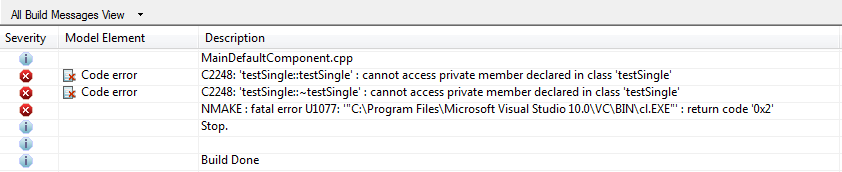
\includegraphics[width=0.99\textwidth]{content/pictures/tests/singleton/error1}
	\label{pic:bild}
	\caption{Fehler beim Zugriff auf privaten Konstruktor}
\end{figure}
  \item[2.]
  Weiterhin muss überprüft werden, ob man von einem bestehenden Singleton-Objekt eine Kopie erzeugen kann. Ist dies möglich, scheitert dieser Test, denn ein Singleton-Objekt darf nicht kopiert werden. Der Copy-Konstruktor muss auch private sein.
  \begin{itemize}
  	\item{Durchführung:}
  	In Rhapsody wurde versucht, eine Instanz der Singleton-Klasse einer Variablen
  	zuzuordnen.
  	\item{Ergebnis:}
  	Der Build in Rhapsody ist fehlgeschlagen, da der Kopierkonstruktor private
  	ist.
  	Der Test ist erfolgreich.
  \end{itemize}
  
 \begin{figure}[!htbp]
	\centering
	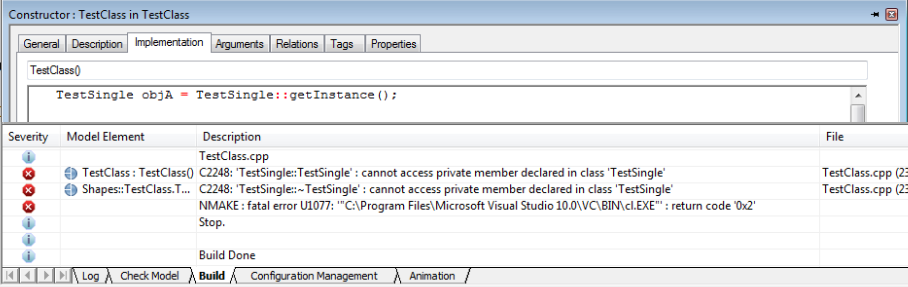
\includegraphics[width=0.99\textwidth]{content/pictures/tests/singleton/KopierError1}
	\label{pic:bild}
	\caption{Fehler bei Kopier-Konstruktor}
\end{figure}
  
  \item[3.]
  Ein weiterer Test ist, dass geprüft werden muss, ob es möglich ist, ein Singleton-Objekt zur Laufzeit zu zerstören. Das Singelton-Objekt wird erst am Ende der Programmlaufzeit freigegeben. Kann das Objekt schon vorher zerstört werden, schlägt der Test fehl. Der Destruktor muss auch als private deklariert sein.
  \begin{itemize}
  	\item{Durchführung:}
  	In Rhapsody wurde versucht, ein Singleton-Object zur Laufzeit zu zerstören.
  	\item{Ergebnis:}
  	Der Build in Rhapsody ist fehlgeschlagen, da der Destruktor pirvate ist. Der
  	Test ist erfolgreich.
  \end{itemize}
  \begin{figure}[!htbp]
	\centering
	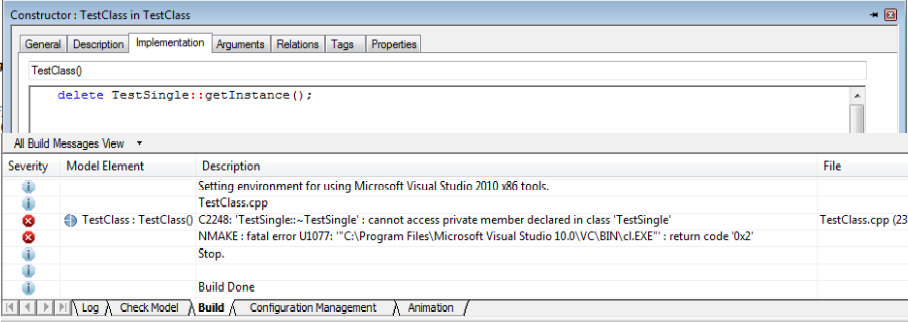
\includegraphics[width=0.99\textwidth]{content/pictures/tests/singleton/deleteError1}
	\label{pic:bild}
	\caption{Fehler beim Löschen des Objekts}
\end{figure}

  \item[4.]
  Möchte man von außerhalb ein Objekt der Singleton-Klasse implementieren, muss dies über die einzige öffentliche Methode der Singleton-Klasse "GetInstance()" passieren. Hierbei wird ein neues Objekt angelegt, sofern noch keins vorhanden war, ansonsten wird einfach das "alte" Objekt zurückgegeben.
  \begin{itemize}
  	\item{Durchführung:}
  	In Rhapsody wird zweimal eine Singleton-Instanz angefordert.
  	\item{Ergebnis:}
  	Der Build in Rhapsody ist erfolgreich. Beim ersten Anfordern einer
  	Singleton-Insatnz wurde eine neue Instanz erstellt, beim zweiten Aufruf wurde
  	die bestehende Instanz zurückgegeben.
  	Der Test ist erfolgreich.
  \end{itemize}
  
  \item[5.]
  Hat der Benutzer selbst eine GetInstance-Methode implementiert, muss Rhapsody bei der Erzeugung des Projektes einen Fehler ausgeben und die Erzeugung abbrechen.
  \begin{itemize}
  \item{Durchführung:}
  In Rhapsody wurde versucht, einer Klasse, die bereits eine getInstance()
  Methode beinhaltet, den Stereotyp <<Singleton>> zuzuordnen.
  \item{Ergebnis:}
  Der Build in Rhapsody ist nicht fehlgeschlagen. Der Test ist nicht
  erfolgreich.
  \end{itemize}
  \begin{figure}[!htbp]
	\centering
	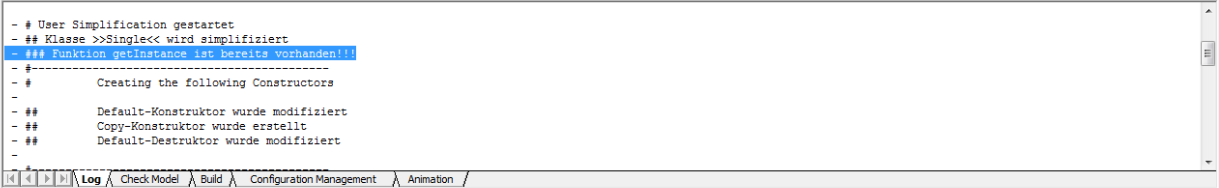
\includegraphics[width=0.999\textwidth]{content/pictures/tests/singleton/getinstanceerror1}
	\label{pic:bild}
	\caption{Fehler bei vorhandener getInstance-Methode}
\end{figure}

  \item[6.]
  Nachdem das Singelton-Objekt mithilfe der getInstance()-Methode erzeugt wurde, liefert diese Methode stets die gleiche Instanz der Singleton-Klasse zurück. 
  \begin{itemize}
  	\item{Durchführung:}
  	In Rhapsody wurden mehrere Singleton-Instanzen angefordert.
  	\item{Ergebnis:}
  	Der Build in Rhapsody war erfolgreich. Bei jeder angeforderten Instanz
  	wurde der gleiche Pointer zurückgegeben. Der Test ist erfolgreich.
  \end{itemize} 
  \begin{figure}[!htbp]
	\centering
	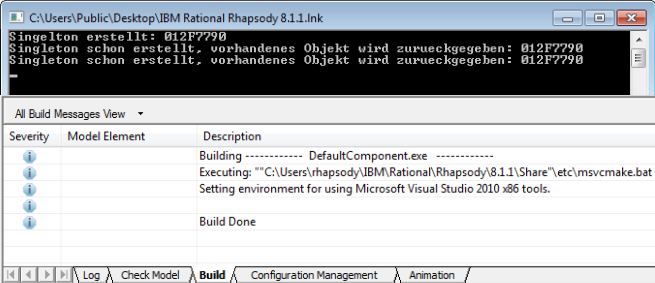
\includegraphics[width=0.9\textwidth]{content/pictures/tests/singleton/HappyDay1}
	\label{pic:bild}
	\caption{Happy-Day bei der Simplification von Singleton}
\end{figure}
 
\end{description}

\section{Observer}

Um sicherzustellen, dass das Observer Pattern richtig implementiert worden ist, müssen neben dem Behandeln der Compiler-Fehler und Warnungen folgende Testfälle manuell überprüft werden: 

\begin{description}

	\item[1.]
	Hat der Benutzer bereits eine Klasse namens Observer oder Subject oder deren Methoden implementiert, muss Rhapsody die Simplification mit Fehlermeldung abbrechen.
	
	\item[2.]
	Wenn der Benutzer nur eine der Observer/Subject Klassen modelliert hat, muss Rhapsody das Programm übersetzen, aber eine entsprechende Warnung ausgeben.
	
	\item[3.]
	Mehrere Observer werden am Subject registriert, danach wird die Anzahl der registrierten Observer überprüft und muss mit der eingegebenen Anzahl übereinstimmen.

	\item[4.]
	Mehrere Observer werden am Subject registriert, danach wird eine bestimmte Anzahl wieder gelöscht. Die Anzahl der registrierten Observer muss den Anfangs registrierten minus den gelöschten Observern entsprechen. Desweiteren darf kein Fehler passieren, wenn versucht wird, einen Observer zu löschen, wenn gar keine Observer registriert wurden.

\end{description}


\section{Guarded Call}

Auch für das letzte Pattern sind einige Tests nötig. Viele verschiedene Faktoren
haben Einfluss auf die Simplification.
\begin{description}

	\item[1.]
	Die ersten Tests sind wie bei den anderen Pattern die Namenskonvention. Hier
	wird überprüft ob der Name für das Attribut bereits vergeben ist. Wenn dies der
	Fall ist, soll eine Meldung gezeigt werden. So kann der Benutzer den Namen
	anpassen.
	
	\item[2.]
	Wenn der Name des Attributs noch frei ist muss überprüft werden ob der Typ der
	Variable auch richtig gesetzt ist. Da es sich hier um eine Variable vom Typ
	OMOSMutex* handelt. Der Variable muss auch der richtige Wert zugewiesen
	werden. Es soll die Rhapsody mutex verwendet werden. (siehe Beschreibung
	Guarded Call)
	
	\item[3.]
	Die Funktionen, die vom Benutzer erstellt wurden müssen in eine andere Funktion
	kopiert werden. (Der Inhalt der Funktion) \\
	Es muss geprüft werden, ob der Inhalt kopiert wurde und ob die Wrapper-Funktion
	funktioniert.
	
	\item[4.]
	Der Funktionsname muss geprüft werden. An die Benutzerfunktionen wird das Wort
	"Guarded" dran gehängt. Wenn eine Funktion schon diese Endung hat, darf die
	Funktion nicht weiter bearbeitet werden. Es folgt wieder eine Meldung an den
	Benutzer.
	
	\item[5.]
	Es muss geprüft werden, ob der Funktionsaufruf von einem try, catch Block
	eingeschlossen wird. 
	
	\item[6.]
	Da immer eine ganze Funktion gesperrt wird, muss geprüft werden ob diese
	Funktion auch wirklich gesperrt ist. Kein anderer Thread darf Zugriff auf die
	gesperrte Funktion haben. 
	
	\item[7.]
	Ein weiterer wichtiger Test ist die Prüfung der Rekursivität der Rhapsody
	mutex. schreib da bitte noch was dazu eric\ldots
	
	\item[8.]
	Funktionen mit Rückgabewerte müssen geprüft werden. Hier gibt es zwei Fälle.
	Primitive Datentypen und Objekte. Hier vllt auch noch kurz was eric\ldots
	
	
\end{description}
